% Current source snapshots: data/occlusion/summary_by_{system,segment}.csv.
\WIPsubsection{Instrument Occlusion}
Instrument masks covered shafts, wrists, and jaws in the left endoscopic view. Occlusion was sampled at one frame per second. The main comparison included three 3 mm recordings and four 8 mm recordings; the mixed-instrument May 28 pilot was excluded.

The median of the recording medians was 10.39\% with 3 mm instruments and 23.93\% with 8 mm instruments (Table~\ref{tab:occlusion}). With occlusion below 1\% excluded, the corresponding values were 10.71\% and 24.42\%. The pooled-frame histogram used this latter filter and had medians of 11.0\% and 25.1\% (Fig.~\ref{fig:occlusion}). These summaries describe different denominators and are not suturing-only comparisons.

\begin{table}[tbp]
\centering
\caption{Occlusion summaries for the main recordings.}
\label{tab:occlusion}
\small
\begin{tabularx}{\linewidth}{@{}Xrr@{}}
\toprule
Measure & 3 mm & 8 mm \\
\midrule
Recordings, $n$ & 3 & 4 \\
Frames in histogram, $n$ & 28,822 & 21,102 \\
Median of recording medians, \% & 10.39 & 23.93 \\
Range of recording medians, \% & 10.25--11.31 & 22.86--26.50 \\
Median of filtered recording medians, \% & 10.71 & 24.42 \\
Pooled filtered-frame median, \% & 11.0 & 25.1 \\
\bottomrule
\end{tabularx}
\par\smallskip
\begin{minipage}{\linewidth}\footnotesize
Dark frames were excluded. Filtered summaries additionally excluded occlusion below 1\%. Recordings, rather than frames, represent the case-level comparison. No significance test is reported.
\end{minipage}
\end{table}

\begin{figure*}[tbp]
\centering
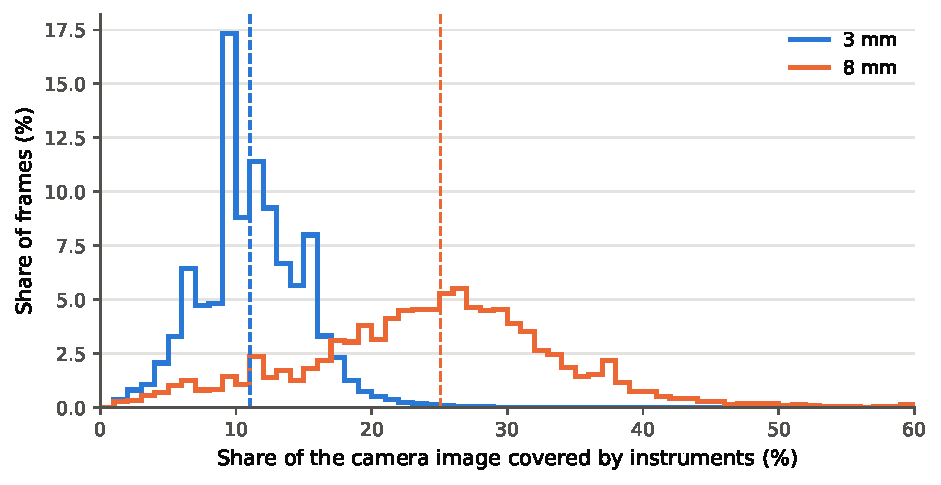
\includegraphics[width=.78\textwidth]{figures/results/occlusion_distribution.pdf}\par\smallskip
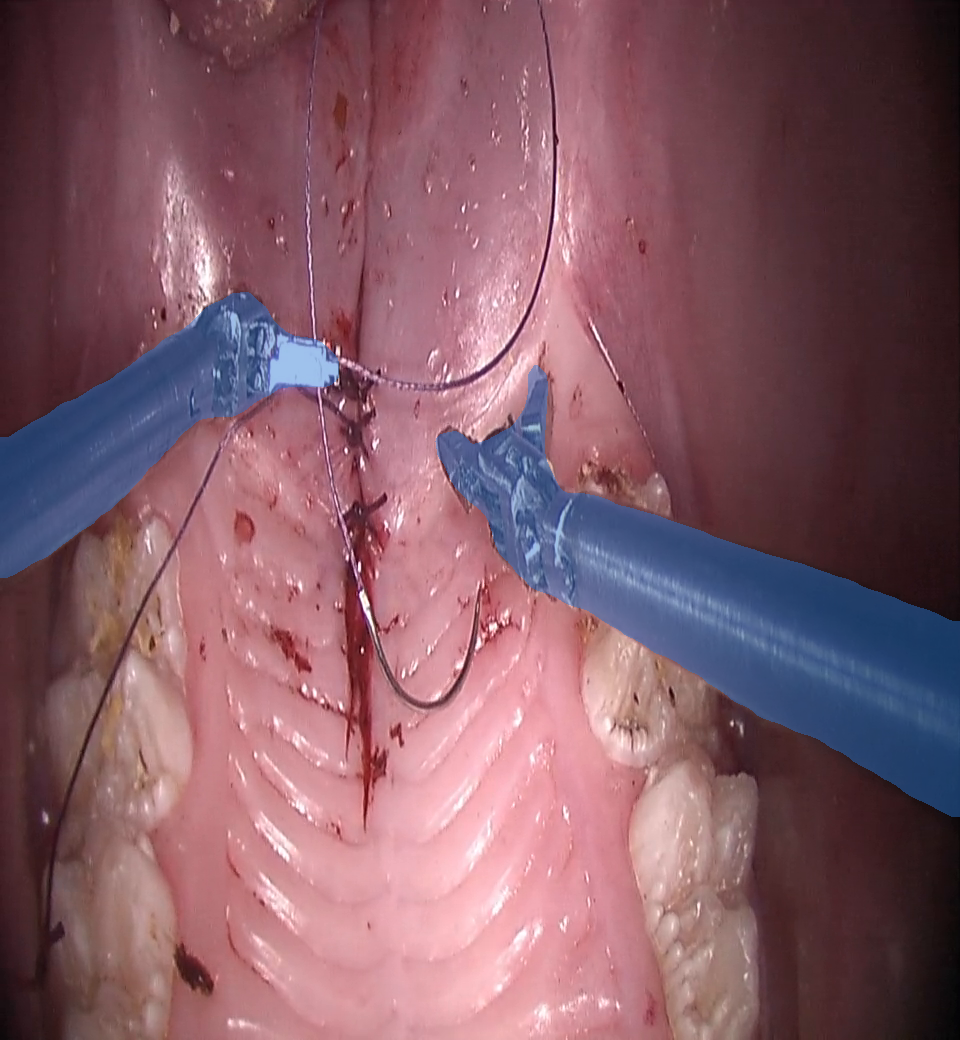
\includegraphics[width=.23\textwidth]{figures/results/occlusion_example_3mm.png}\hspace{.04\textwidth}
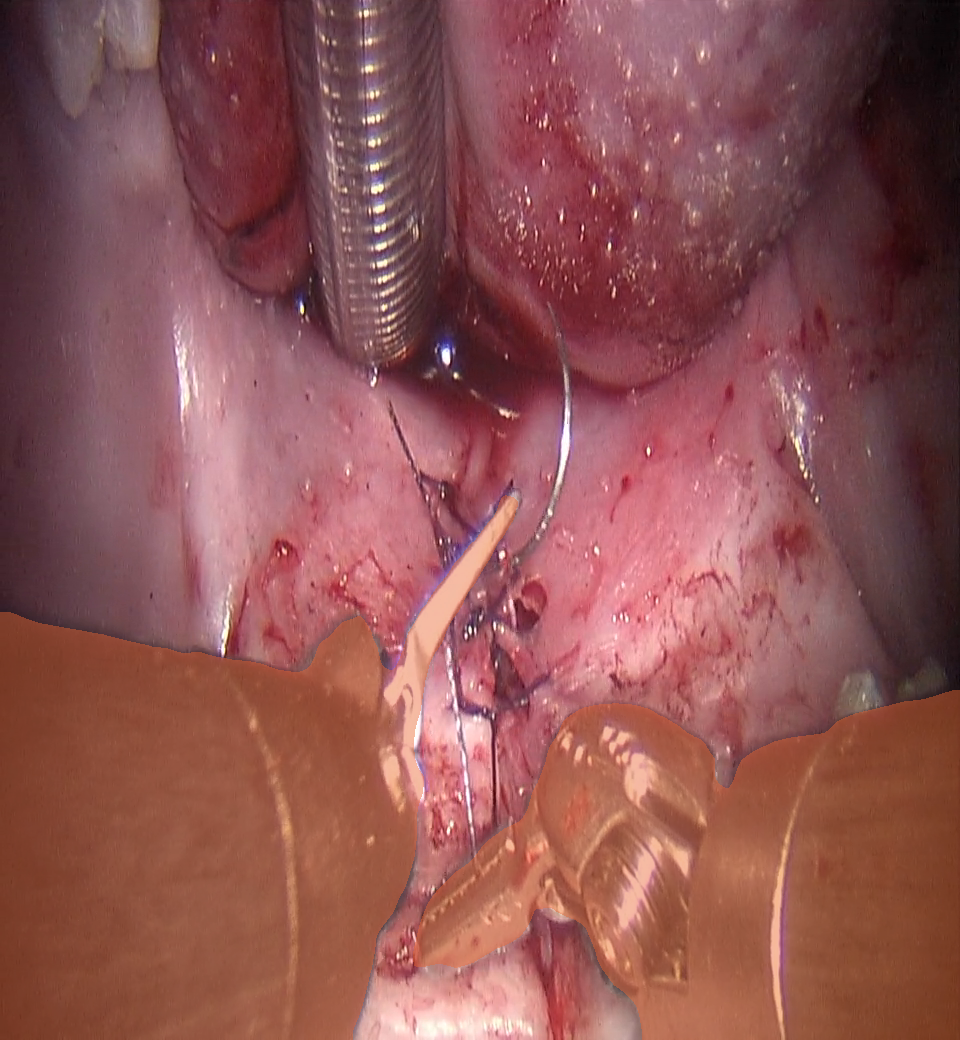
\includegraphics[width=.23\textwidth]{figures/results/occlusion_example_8mm.png}
\caption{Instrument occlusion in the main recordings. Top: pooled frames with at least 1\% occlusion; dashed lines mark medians. The plotted axis ends at 60\%. Bottom: selected suturing examples with instrument masks, 3 mm on the left (11\% occlusion) and 8 mm on the right (30\%). These examples were selected by eye and were not matched for camera distance or task position.}
\label{fig:occlusion}
\end{figure*}

\begin{itemize}
\item Camera distance varied; lower image obstruction does not isolate instrument diameter from camera placement.
\item The segmentation test used 30 held-out frames from the same six training-source recordings. Median intersection-over-union was 0.921 for 3 mm and 0.973 for 8 mm instruments. May 29 was outside those six recordings.
\item \textbf{[Confirm May 29 mask quality and distinguish pooled-frame summaries from case-level estimates in the final interpretation.]}
\end{itemize}
